\section{Air quality visualizations}
The problem of making the air quality problem visible to the general population has been addressed before, from map based representations, to wearable devices and in-city displays. These approaches contemplate new or known was to tackle the problem of air quality, and therefore; making the invisible visible.

\subsection{Table based}
The most basic representation of air quality data is as tabular data, generally including some colors to indicate the quality level of the measurement as shown in figure \ref{fig:table_based_visualization}. From these kind of representations is easy to read information from multiple places when the user is familiar to the values. But, as stated before, this representations have many drawbacks. 

\begin{figure}[H]
\begin{adjustbox}{width=1\textwidth,center=\textwidth}
  \centering
  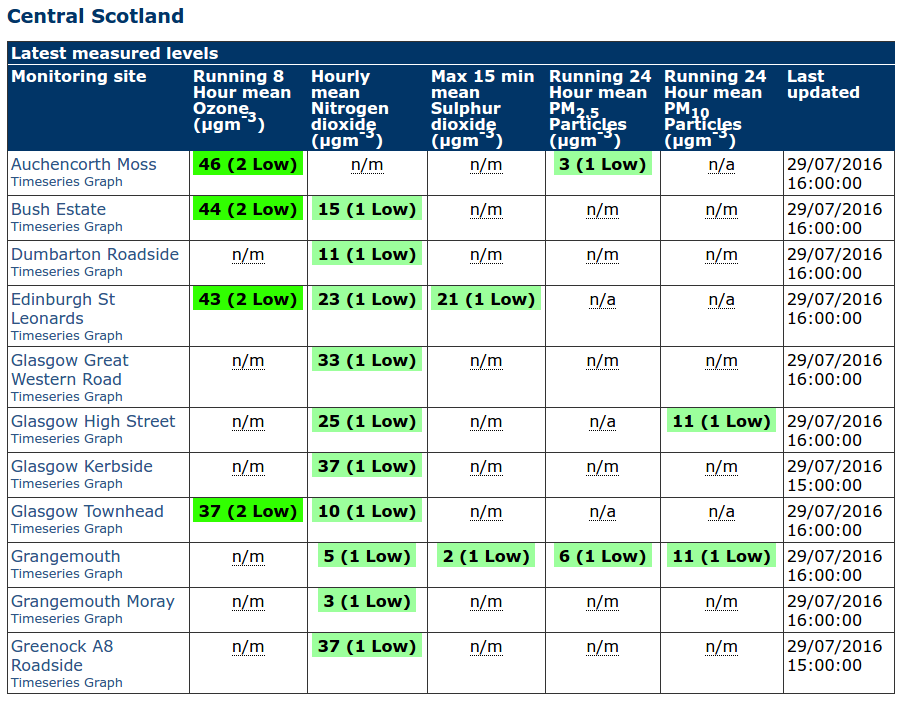
\includegraphics[scale=1]{images/tabular_data.png}
\end{adjustbox}
  \caption[Tabular visualization]{Tabular visualization \cite{DepartmentforEnvironment}}
  \label{fig:table_based_visualization}
\end{figure}

\subsection{Map based}
Through maps; people is able to understand where the measurements are coming from. Some representations include color indicators to show how good or bad the measurements are. However; it is unlikely that one is interested in the measurements for all Scotland's regions,, it is time consuming to browse manually to the desired zone to explore the current values, and it is hard to correctly visualize overlaid numeric data on small screens.

\begin{figure}[H]
\begin{adjustbox}{width=1\textwidth,center=\textwidth}
  \centering
  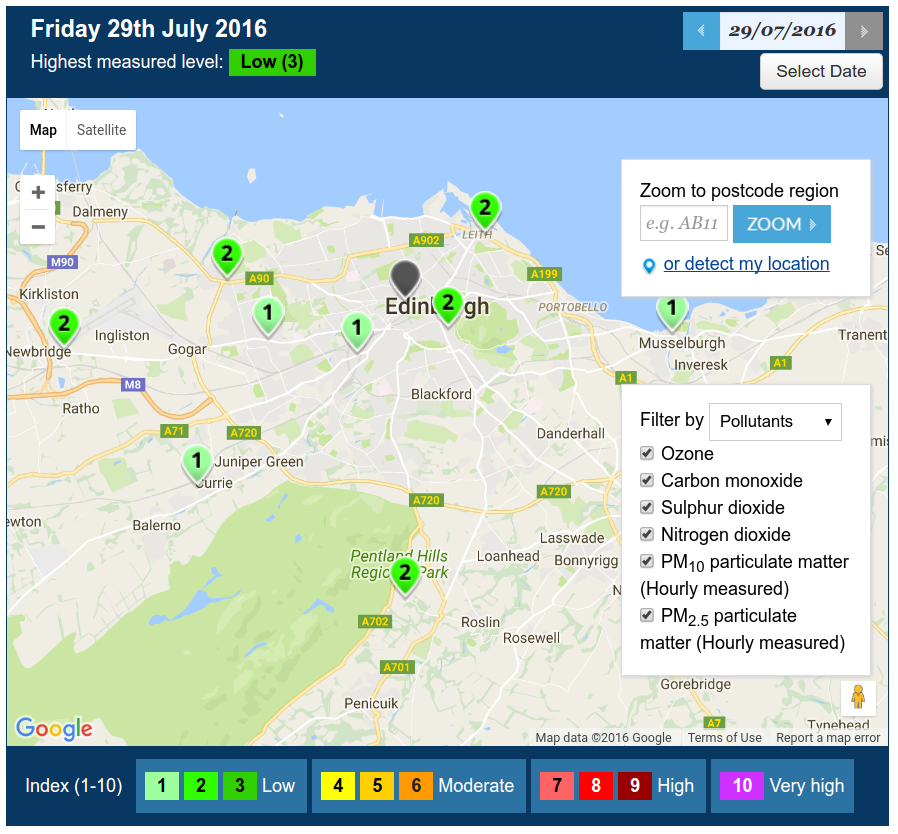
\includegraphics[scale=.30]{images/map_visualization.png}
\end{adjustbox}
  \caption[Map-based visualization]{Map-based visualization \cite{Scottishairquality.co.uk2016}}
  \label{fig:web_based_desktop_visualization}
\end{figure}


\subsection{Line based}
The inAir project \cite{Kim2013} utilizes a line graph to represent indoor particle matter count over a defined period of time. Their findings suggested that this approach enables users to reflect on their behaviors and air quality status, persuading them to modify their practices to decrease their exposure to air pollution.

\begin{figure}[H]
\begin{adjustbox}{width=1\textwidth,center=\textwidth}
  \centering
  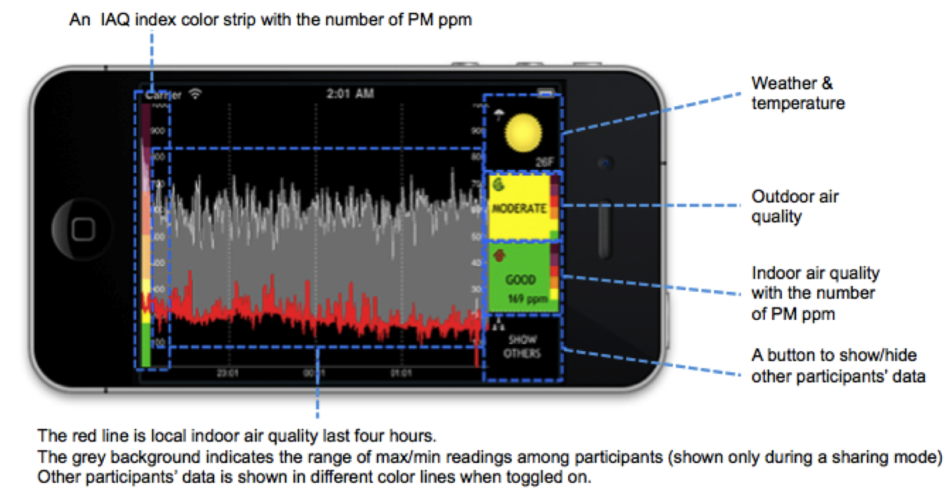
\includegraphics[scale=1]{images/InAir.png}
\end{adjustbox}
  \caption[inAir project: line-based visualizations]{inAir: line-based visualization\cite{Kim2013}.}
  \label{fig:line_based_inAir}
\end{figure}


\subsection{Photo based}
Photo-based representations as proposed by Lin \cite{Lin2014}, allow people to understand levels of pollution by taking pictures of the current environment. The pictures are later adjusted using a filter that represents the air quality status (NO2) at that location. This serves as a playful and habitual way to visualize air quality. On the other hand, this project only aggregates nitrogen dioxide readings, excluding other pollutants that may be pertinent, as well as not going further to indicate what should a person do given the pollution levels.

\begin{figure}[H]
\begin{adjustbox}{width=.8\textwidth,center=\textwidth}
  \centering
  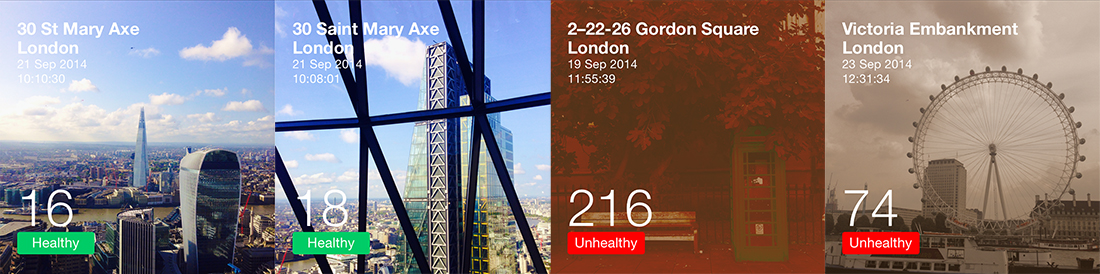
\includegraphics[scale=.4]{images/instaNO2.jpg}
\end{adjustbox}
  \caption[InstaNO2 project: photo-based visualizations]{InstaNO2: photo-based visualizations \cite{Lin2014}.}
  \label{fig:photo_based_instaNO2}
\end{figure}

\subsection{Tangible approaches}
Other approaches have made use of tangible objects to visualize air pollution in a more engaging way. The Human sensor project \cite{InvisibleDust2016} employs wearable art and in-city performances to reveal changes in pollution. Similarly, WearAir \cite{Kim2010}, is an expressive T-shirt that senses VOCs and expresses the readings making use of embedded lights. Kuznetsov et al. \cite{Kuznetsov2011} developed glowing balloons with air quality sensors for users to explore urban air quality. The IBM think exhibit \cite{IBM2012} is a 123-foot long digital wall display located in New York city which renders art patterns and real time streaming visualizations showing air quality data as well as traffic flow, energy, and water usage. This is intended to be an immersive in-city experience for users to explore and understand the role of data in the world. Tangible approaches are useful because the evoke curiosity and surprise, also, it is easy to gain an insight of what is happening. In contrast, they are not intended for personal day to day usage but as a way of expression and art. 

\begin{figure}[H]
\begin{adjustbox}{width=.8\textwidth,center=\textwidth}
  \centering
  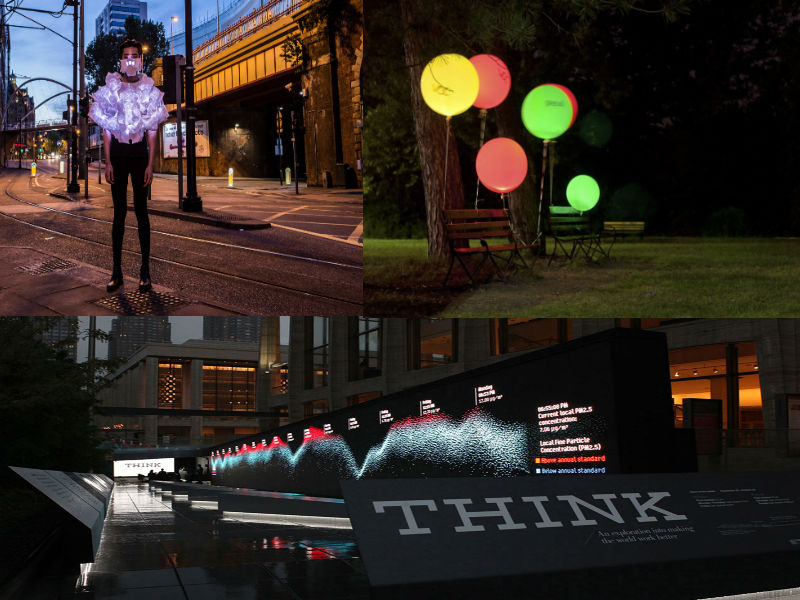
\includegraphics[scale=.4]{images/think_human_sensor_balloons.jpg}
\end{adjustbox}
  \caption[Tangible visualizations]{The human-sensor on the top-left \cite{InvisibleDust2016}, glowing balloons on the top-right \cite{Kuznetsov2011}, and IBM think on the bottom \cite{IBM2012}.}
  \label{fig:photo_based_instaNO2}
\end{figure}

